\documentclass[11pt]{article}

\usepackage[margin=1in]{geometry}
\usepackage{amsmath,amssymb,amsthm,amsfonts}
\usepackage{algorithmic,algorithm}
\usepackage{bbm}
\usepackage{booktabs}
\usepackage{graphicx}
\usepackage{microtype}
\usepackage[authoryear,round]{natbib}
\usepackage[hidelinks]{hyperref}
\usepackage{url}

\newtheorem{theorem}{Theorem}
\newtheorem{lemma}{Lemma}
\newtheorem{proposition}{Proposition}
\newtheorem{corollary}{Corollary}
\newtheorem{definition}{Definition}
\newtheorem{assumption}{Assumption}
\newtheorem{remark}{Remark}
\DeclareMathOperator*{\argmax}{arg\,max}
\DeclareMathOperator*{\argmin}{arg\,min}
\newcommand{\E}{\mathbb E}
\newcommand{\Var}{\operatorname{Var}}
\setlength{\emergencystretch}{2em}

\title{Mixtures of Generalized Regression Models with\\
Component-Specific Response Families}
\author{Samyajoy Pal}
\date{}

\begin{document}

\maketitle

\begin{abstract}
Finite mixtures of generalized linear model (GLM) regressions usually vary regression
parameters across latent components while retaining one response family for all
components.  This restriction can confound latent heterogeneity in covariate
effects with heterogeneity in tail weight, dispersion, skewness, or zero
inflation.  We introduce a generalized regression-mixture framework in which each component
may have its own response family, link, nuisance parameters, and sparse
regression vector.  Estimation uses a penalized generalized
expectation-maximization (EM) algorithm, and the number and composition of
components are selected from support-compatible family tuples by exhaustive or
beam search using the Bayesian information criterion (BIC).  For a fixed
regular family tuple, we establish identifiability, consistency and asymptotic
normality, characterize the local limit under lasso penalization, and prove
generalized-EM monotonicity.  We derive the observed information through Louis' identity and
provide closed-form derivative blocks for fourteen continuous, positive,
binary, count, zero-inflated, and skew families.  Simulations show increasing
recovery of non-identical family structures, substantial reductions in false
selection under componentwise penalization, and close agreement between
analytical Louis and numerical-Hessian standard errors.  Applications to
Parkinson's telemonitoring and RAND health-utilization data identify
non-identical mixtures.  In the RAND analysis, a Poisson--negative-binomial
mixture is selected in three independent splits and in the full sample; a
selection-aware bootstrap supports a stable, strongly overdispersed minority
component.  We state explicitly the regularity boundary between fixed-model
likelihood inference and the nonregular problems created by family search,
component selection, and penalization.
\end{abstract}

\noindent\textbf{Keywords:} finite mixture regression; generalized regression
model; heterogeneous response families; penalized expectation-maximization;
variable selection; Louis information; model selection.

\section{Introduction}
\label{sec:introduction}

Finite mixture models provide a natural representation of unobserved
heterogeneity: each observation arises from one of several latent
subpopulations, and the observed law averages over the unknown membership
\citep{mclachlan2000finite}.  Mixtures of regressions extend this principle by
allowing the regression relationship itself to vary across latent components.
In parallel, generalized linear models (GLMs) unify regression for continuous,
binary, count, and positive responses through a response family and link
function \citep{nelder1972glm,mccullagh1989glm}.  Their combination has become
an important tool for latent-class regression, clustering, and overdispersion
\citep{leisch2004flexmix,grun2007fitting,grun2008finite}.
We use \emph{generalized regression} in the broader link-based sense:
classical exponential-family GLMs are included, while Student-$t$, lognormal,
and skew-normal components extend beyond the strict GLM class.

Most finite mixtures of GLMs nevertheless impose a common response family
across components.  Components may have different intercepts, regression
coefficients, or dispersion parameters, but all are Gaussian, all are Poisson,
or all are negative binomial.  This convention is computationally convenient,
yet it is scientifically restrictive.  A count population may contain a
regular-use subpopulation with approximately Poisson variation and a smaller
subpopulation with severe residual overdispersion.  A continuous response may
combine a central approximately symmetric group with a heavy-tailed or skewed
group.  Adding more components from one family can approximate such behavior,
but it also confounds the number of latent subpopulations with the shape needed
to accommodate misspecification.

Several neighboring literatures address parts of this problem.  Flexible
mixture-regression software permits modular component models
\citep{leisch2004flexmix,grun2007fitting}; mixture-of-experts models allow
covariate-dependent routing among local predictors \citep{jacobs1991experts};
and penalized mixture regressions allow component-specific variable selection
\citep{khalili2007variable,stadler2010l1}.  Robust, skew, zero-inflated, and
overdispersed mixtures relax particular distributional assumptions
\citep{azzalini1985skew,lambert1992zip}.  What remains comparatively
underdeveloped is an integrated regression framework that searches over
\emph{non-identical} response-family tuples, performs sparse estimation within
the selected components, and supplies a common observed-information calculation
despite family-specific nuisance parameters.

This paper makes five contributions.  First, we formulate a mixture of
generalized regression models in which response families, links, nuisance
parameters, and coefficient supports may differ by component.  Second, we
develop a penalized generalized expectation-maximization algorithm and a
support-aware search over
the number and composition of components.  Third, for a fixed regular family
tuple we give a careful likelihood theory: identifiability, existence and
consistency of the maximum likelihood estimator, asymptotic normality,
generalized-EM monotonicity, and the local effect of lasso penalization.  Fourth,
we combine Louis' identity \citep{louis1982information} with family-specific
derivative blocks, avoiding a large numerical Hessian for the families used in
our experiments.  Fifth, we evaluate structural recovery, prediction,
component-specific sparsity, standard errors, and coverage in simulations and
in continuous and count applications.

The scope of the theory is deliberate.  Finite mixtures are singular when
components coincide, weights vanish, or an overfitted model contains the truth;
family comparisons may also meet at boundaries, as Poisson does with negative
binomial.  Ordinary fixed-dimensional Wald theory does not cover these cases,
nor does it automatically survive lasso selection
\citep{knight2000asymptotics,drton2017sbic}.  We therefore distinguish
fixed-model likelihood inference from the empirical family search and use a
selection-aware bootstrap in the principal count application.  This distinction
is not merely technical: it prevents a computationally convenient standard
error from being given an inferential interpretation it does not possess.

The remainder of the paper is organized as follows.  Sections
\ref{sec:methodology} and \ref{sec:theory} present the model, estimation,
search, and theory.  Section~\ref{sec:results} reports simulations and two
applications.  Section~\ref{sec:discussion} discusses the implications and
limitations.  Appendix~\ref{app:louis_mstep} gives the family-level analytical
Louis blocks and weighted M-step equations.  Complete simulation settings and
additional application tables are provided in the Supplementary Material.

\section{Methodology}
\label{sec:methodology}

The methodology has three layers: the fixed family-tuple likelihood model, the
penalized expectation-maximization computation used to fit a candidate, and the
model-search device used to compare candidate tuples.  We state these layers
separately because they have different mathematical status and lead to
different inferential claims.

\subsection{Scope of the methodology}

We first define the statistical object studied in the paper and separate three
regimes that require different inferential arguments.

First, the regular fixed-model regime treats the number of components \(K\) and
the ordered tuple of component families
\[
    \mathfrak m=(d_1,\ldots,d_K)
\]
as fixed.  The true parameter is assumed to be an interior point, no two
components coincide, mixing weights are bounded away from zero, and the Fisher
information is nonsingular after a labeling convention is imposed.  The
identifiability, consistency, asymptotic normality, Louis-information, and EM
monotonicity results below are proved for this regime.

Second, penalized estimation is used as a computational and regularization
device.  Penalization changes the distributional limit of the estimator unless
the tuning parameter is asymptotically negligible at the \(n^{-1/2}\) scale.
For this reason, the likelihood-based standard errors in this paper target the
unpenalized estimator, or a post-selection refit on a fixed selected model, not
the raw lasso estimator.

Third, choosing \(K\), choosing the family tuple, and comparing nested families
such as Poisson inside negative binomial are model-selection and nonregular
problems.  We describe the procedure used in the computations, but the regular
asymptotic theorems do not by themselves justify ordinary Wald inference after
family search, component-number search, or boundary selection.

\subsection{Fixed family-tuple model}

Let \((Y_i,X_i)\), \(i=1,\ldots,n\), be independent observations from the joint
law of \((Y,X)\), where \(Y\in\mathcal Y\subseteq\mathbb R\) and
\(X\in\mathcal X\subseteq\mathbb R^p\).  The first component of \(X\) is an
intercept.  For a fixed model \(\mathfrak m=(d_1,\ldots,d_K)\), assume that all
families in \(\mathfrak m\) are dominated by a common sigma-finite measure
\(\nu\) on \(\mathcal Y\).  This excludes mixtures whose component laws live on
incompatible supports unless a common dominating measure has been explicitly
specified.

For family \(d\), let
\[
    f_d(y;\mu,\gamma)
\]
denote its density or mass function with respect to \(\nu\), where
\(\mu\in\mathcal M_d\) is the systematic location or mean-like parameter and
\(\gamma\in\Gamma_d\) is a finite-dimensional nuisance parameter.  The inverse
link is denoted by
\[
    h_d(\eta)=g_d^{-1}(\eta).
\]
For component \(k\), define
\[
    q_k(y\mid x;\beta_k,\gamma_k)
    =
    f_{d_k}\{y;h_{d_k}(x^\top\beta_k),\gamma_k\}.
\]
The conditional mixture density is
\[
    p_\theta(y\mid x)
    =
    \sum_{k=1}^K \pi_k q_k(y\mid x;\beta_k,\gamma_k),
    \qquad
    \pi_k>0,\quad \sum_{k=1}^K\pi_k=1,
\]
where
\[
    \theta=\{(\pi_k,\beta_k,\gamma_k):k=1,\ldots,K\}\in\Theta_{\mathfrak m}.
\]
The family labels \(d_k\) are part of the model \(\mathfrak m\), not continuous
parameters.

Because finite mixtures are invariant under relabeling, \(\theta\) is
identifiable at best up to permutations that preserve the multiset of
components.  In local asymptotic statements we work in a labeled neighborhood of
the true parameter, for example by imposing a deterministic ordering rule.  All
global identifiability statements are understood modulo label permutations.

\subsection{Observed and penalized likelihoods}

For fixed \(\mathfrak m\), the observed log-likelihood is
\[
    \ell_n(\theta)
    =
    \sum_{i=1}^n
    \log p_\theta(Y_i\mid X_i).
\]
The unpenalized estimator is
\[
    \hat\theta_n
    \in
    \argmax_{\theta\in\Theta_{\mathfrak m}}\ell_n(\theta).
\]

For regularized estimation, let \(\beta_{k,-0}\) denote the non-intercept
coordinates of \(\beta_k\).  We use penalties of the form
\[
    P_n(\theta)
    =
    \sum_{k=1}^K \lambda_{n,k}\rho_k(\beta_{k,-0}),
\]
where \(\rho_k\) may be ridge, lasso, or elastic-net.  The penalized estimator
is
\[
    \hat\theta_{n,\lambda}
    \in
    \argmax_{\theta\in\Theta_{\mathfrak m}}
    \{\ell_n(\theta)-P_n(\theta)\}.
\]
The intercept is not penalized.  This convention follows standard sparse
regression practice \citep{tibshirani1996lasso} and is used throughout.

\subsection{Expectation-maximization representation}

Introduce latent variables \(Z_i\in\{1,\ldots,K\}\) with
\(\Pr(Z_i=k)=\pi_k\).  Given \(Z_i=k\), the conditional density of \(Y_i\) is
\(q_k(Y_i\mid X_i;\beta_k,\gamma_k)\).  The complete-data log-likelihood is
\[
    \ell_{c,n}(\theta)
    =
    \sum_{i=1}^n\sum_{k=1}^K
    \mathbbm 1(Z_i=k)
    \{\log\pi_k+\log q_k(Y_i\mid X_i;\beta_k,\gamma_k)\}.
\]
Given the current parameter \(\theta^{(t)}\), the posterior responsibilities are
\[
    \tau_{ik}^{(t)}
    =
    \frac{
        \pi_k^{(t)}q_k(Y_i\mid X_i;\beta_k^{(t)},\gamma_k^{(t)})
    }{
        \sum_{\ell=1}^K
        \pi_\ell^{(t)}
        q_\ell(Y_i\mid X_i;\beta_\ell^{(t)},\gamma_\ell^{(t)})
    }.
\]
The penalized EM objective is
\[
    Q_{P,n}(\theta\mid\theta^{(t)})
    =
    \sum_{i=1}^n\sum_{k=1}^K
    \tau_{ik}^{(t)}
    \{\log\pi_k+\log q_k(Y_i\mid X_i;\beta_k,\gamma_k)\}
    -
    P_n(\theta).
\]
The resulting construction follows the EM principle of
\citet{dempster1977em}.  The mixing proportions have the closed-form update
\[
    \pi_k^{(t+1)}
    =
    n^{-1}\sum_{i=1}^n\tau_{ik}^{(t)}.
\]
The remaining update decomposes by component:
\[
    (\beta_k^{(t+1)},\gamma_k^{(t+1)})
    \in
    \argmax_{\beta_k,\gamma_k}
    \left[
    \sum_{i=1}^n\tau_{ik}^{(t)}
    \log q_k(Y_i\mid X_i;\beta_k,\gamma_k)
    -
    \lambda_{n,k}\rho_k(\beta_{k,-0})
    \right].
\]
When this maximization is exact, the algorithm is an EM algorithm for the
penalized objective.  When the component update is only improved, but not
globally maximized, the algorithm is a generalized EM algorithm.  The
monotonicity result below requires the explicit ascent condition
\[
    Q_{P,n}(\theta^{(t+1)}\mid\theta^{(t)})
    \ge
    Q_{P,n}(\theta^{(t)}\mid\theta^{(t)}).
\]

\subsection{Model search}

Let \(\mathcal D\) be a finite collection of candidate response families.  We
consider only family tuples whose supports are compatible with the observed
support of \(Y\).  For a fitted model \(\mathfrak m\), define
\[
    \mathrm{BIC}(\mathfrak m)
    =
    -2\ell_n(\hat\theta_{\mathfrak m})
    +
    a_{\mathfrak m}\log n,
\]
where BIC denotes the Bayesian information criterion and
\(a_{\mathfrak m}\) is the number of free parameters in the fixed model
\citep{schwarz1978dimensions}.
Penalized fits are used as a screening and regularization device.  For a
lasso-selected or elastic-net-selected support, the final likelihood score is
computed by refitting the same family tuple without penalty while holding the
component-specific active sets fixed.  If
\(\hat S_k=\{j>0:\hat\beta_{kj}\neq0\}\) is the selected non-intercept support
for component \(k\), the refitted model uses the parameter count
\[
    \hat a_{\mathfrak m}
    =
    (K-1)
    +K
    +
    \sum_{k=1}^K
    |\hat S_k|
    +
    \sum_{k=1}^K\dim(\gamma_k),
\]
where the second term counts the \(K\) component intercepts.  We report the
penalized objective and the unpenalized likelihood of the screening fit, but
rank lasso-selected candidates by the BIC of the unpenalized active-set refit
when the refit converges.  Ridge penalties do not define a sparse active set
and are therefore treated as sensitivity analyses rather than as sources of
post-lasso BIC scores.  The refit BIC is still conditional on the selected
support and family tuple; it is a transparent computational score, not a claim
of valid post-selection inference.

For small candidate spaces we enumerate all unordered family tuples.  For
larger spaces the implementation uses a beam search: tuples of size \(K\) are
expanded from retained tuples of size \(K-1\), fitted by the EM procedure, and
only the best few according to the chosen criterion are carried forward.  The
beam search is a deterministic heuristic conditional on initialization and
random seed; it does not inherit the fixed-model regularity theory.

\section{Theoretical properties}
\label{sec:theory}

We next record the likelihood properties that are used to interpret a fitted
candidate model.  The results are intentionally conditional on a fixed,
regular, identifiable candidate; later family search, component-number
selection, and active-set selection are treated as separate nonregular
operations.

\subsection{Regular fixed-model assumptions}

All results in Sections~\ref{sec:identifiability}--\ref{sec:louis_theory}
condition on a fixed family tuple \(\mathfrak m=(d_1,\ldots,d_K)\).  Write
\(\theta_0\) for the true parameter.

\begin{assumption}[Sampling]
\label{ass:sampling}
The observations \((Y_i,X_i)\), \(i=1,\ldots,n\), are independent and
identically distributed.  Conditional on \(X=x\), the true density of \(Y\) is
\(p_{\theta_0}(y\mid x)\) for some \(\theta_0\in\Theta_{\mathfrak m}\).
\end{assumption}

\begin{assumption}[Parameter space]
\label{ass:param_space}
The parameter space \(\Theta_{\mathfrak m}\) is compact after imposing a
labeling convention.  The true parameter \(\theta_0\) is an interior point of
this labeled parameter space.  There exists \(\pi_{\min}>0\) such that
\(\pi_k\ge \pi_{\min}\) for all \(k\) and all \(\theta\in\Theta_{\mathfrak m}\).
Nuisance parameters are bounded away from degeneracies such as zero variances,
infinite dispersions, and boundary zero-inflation probabilities.
\end{assumption}

\begin{assumption}[Continuity and domination]
\label{ass:continuity}
For each \((y,x)\), \(p_\theta(y\mid x)\) is continuous in \(\theta\).  Moreover
\(\log p_\theta(Y\mid X)\) is dominated by an integrable envelope in a
neighborhood of every \(\theta\in\Theta_{\mathfrak m}\), so that
\[
    \sup_{\theta\in\Theta_{\mathfrak m}}
    \left|
    n^{-1}\ell_n(\theta)
    -
    E_{\theta_0}\log p_\theta(Y\mid X)
    \right|
    \to 0
\]
in probability.
\end{assumption}

\begin{assumption}[Primitive component identifiability]
\label{ass:primitive_component}
For each family \(d\), if
\[
    f_d(y;\mu_1,\gamma_1)=f_d(y;\mu_2,\gamma_2)
    \quad\text{for \(\nu\)-almost every }y,
\]
then \((\mu_1,\gamma_1)=(\mu_2,\gamma_2)\).  The inverse link \(h_d\) is
one-to-one on its domain.  Finally, if \(X^\top b=0\) almost surely, then
\(b=0\).
\end{assumption}

\begin{assumption}[Finite-mixture separability]
\label{ass:mixture_separability}
The collection of component regression densities
\[
    \mathcal Q_{\mathfrak m}
    =
    \left\{
    q_k(\cdot\mid\cdot;\beta,\gamma):
    k=1,\ldots,K,\;(\beta,\gamma)\in\mathcal B_{d_k}\times\Gamma_{d_k}
    \right\}
\]
is \(K\)-identifiable in the following sense.  If two mixtures with at most
\(K\) nonzero components satisfy
\[
    \sum_{r=1}^{m} a_r q_r(y\mid x)
    =
    \sum_{s=1}^{m'} b_s \tilde q_s(y\mid x)
\]
for \(P_X\)-almost every \(x\) and \(\nu\)-almost every \(y\), where
\(a_r,b_s>0\), \(\sum_r a_r=\sum_s b_s=1\), and all atoms on each side are
distinct, then \(m=m'\) and the two sets of weighted atoms are equal up to
permutation.
\end{assumption}

\begin{remark}
Assumption~\ref{ass:mixture_separability} is the nontrivial finite-mixture
identifiability condition.  It is intentionally stated explicitly rather than
hidden behind the phrase ``standard mixture arguments.''  It must be verified
or cited for any family tuple used as a formal model.  It can fail at nested or
boundary cases, for example when an overdispersed family contains a simpler
family as a limiting special case; see \citet{teicher1963identifiability} and
\citet{hennig2000identifiability} for foundational results and regression-mixture
qualifications.
\end{remark}

\subsection{Identifiability}
\label{sec:identifiability}

\begin{lemma}[Component regression identifiability]
\label{lem:component_ident}
Under Assumption~\ref{ass:primitive_component}, for a fixed family \(d\),
\[
    f_d\{y;h_d(x^\top\beta_1),\gamma_1\}
    =
    f_d\{y;h_d(x^\top\beta_2),\gamma_2\}
\]
for \(P_X\)-almost every \(x\) and \(\nu\)-almost every \(y\) implies
\[
    \beta_1=\beta_2,
    \qquad
    \gamma_1=\gamma_2.
\]
\end{lemma}

\begin{proof}
By primitive identifiability of the family, for \(P_X\)-almost every \(x\),
\[
    h_d(x^\top\beta_1)=h_d(x^\top\beta_2),
    \qquad
    \gamma_1=\gamma_2.
\]
Since \(h_d\) is one-to-one,
\[
    x^\top(\beta_1-\beta_2)=0
\]
for \(P_X\)-almost every \(x\).  The full-rank condition in
Assumption~\ref{ass:primitive_component} then gives \(\beta_1=\beta_2\).
\end{proof}

\begin{theorem}[Identifiability of the fixed family-tuple model]
\label{thm:fixed_ident}
Suppose Assumptions~\ref{ass:param_space}, \ref{ass:primitive_component}, and
\ref{ass:mixture_separability} hold.  If
\[
    p_{\theta_1}(y\mid x)=p_{\theta_2}(y\mid x)
\]
for \(P_X\)-almost every \(x\) and \(\nu\)-almost every \(y\), then
\(\theta_1\) and \(\theta_2\) are equal up to a permutation of component
labels.
\end{theorem}

\begin{proof}
Write both sides as finite mixtures of distinct component regression densities.
If any repeated atom occurs within either representation, combine its weights;
Assumption~\ref{ass:param_space} keeps all remaining weights positive.
Assumption~\ref{ass:mixture_separability} implies equality of the weighted
atoms up to permutation.  Therefore, after relabeling,
\[
    \pi_k^{(1)}=\pi_k^{(2)}
    \quad\text{and}\quad
    q_k(\cdot\mid\cdot;\beta_k^{(1)},\gamma_k^{(1)})
    =
    q_k(\cdot\mid\cdot;\beta_k^{(2)},\gamma_k^{(2)}).
\]
Lemma~\ref{lem:component_ident} then gives
\((\beta_k^{(1)},\gamma_k^{(1)})
=
(\beta_k^{(2)},\gamma_k^{(2)})\) for every \(k\).
\end{proof}

\subsection{Existence and consistency}

\begin{theorem}[Consistency of the maximum likelihood estimator]
\label{thm:consistency}
Under Assumptions~\ref{ass:sampling}--\ref{ass:mixture_separability}, an
unpenalized maximizer \(\hat\theta_n\) exists with probability tending to one.
Moreover, after applying the labeling convention,
\[
    \hat\theta_n\to\theta_0
\]
in probability.
\end{theorem}

\begin{proof}
Existence follows from compactness of \(\Theta_{\mathfrak m}\) and continuity of
\(\ell_n(\theta)\).  Define the population criterion
\[
    M(\theta)=E_{\theta_0}\log p_\theta(Y\mid X).
\]
By Assumption~\ref{ass:continuity},
\[
    \sup_{\theta\in\Theta_{\mathfrak m}}
    |n^{-1}\ell_n(\theta)-M(\theta)|
    \to 0
\]
in probability.  For any \(\theta\),
\[
    M(\theta)-M(\theta_0)
    =
    -E_{\theta_0}
    \log\frac{p_{\theta_0}(Y\mid X)}{p_\theta(Y\mid X)}
    \le 0,
\]
with equality if and only if
\[
    p_\theta(Y\mid X)=p_{\theta_0}(Y\mid X)
\]
almost surely.  By Theorem~\ref{thm:fixed_ident} and the imposed labeling
convention, equality holds only at \(\theta=\theta_0\).  Hence \(M\) has a
unique maximizer at \(\theta_0\).  The argmax theorem gives
\(\hat\theta_n\to\theta_0\) in probability.
\end{proof}

\subsection{Regular asymptotic normality}

\begin{assumption}[Local differentiability and information]
\label{ass:local_regular}
In a neighborhood of \(\theta_0\), the labeled parameter can be represented as a
vector in an open subset of \(\mathbb R^r\).  The map
\(\theta\mapsto \log p_\theta(Y\mid X)\) is twice continuously differentiable
in this neighborhood, differentiation may be interchanged with expectation, and
the Fisher information
\[
    I(\theta_0)
    =
    E_{\theta_0}
    \left[
        S_{\theta_0}(Y,X)S_{\theta_0}(Y,X)^\top
    \right],
    \qquad
    S_{\theta}(Y,X)=\nabla_\theta\log p_\theta(Y\mid X),
\]
is finite and nonsingular.
\end{assumption}

\begin{theorem}[Asymptotic normality in the regular fixed model]
\label{thm:asymptotic_normality}
Under Assumptions~\ref{ass:sampling}--\ref{ass:local_regular},
\[
    \sqrt n(\hat\theta_n-\theta_0)
    \Rightarrow
    N\{0,I(\theta_0)^{-1}\}.
\]
\end{theorem}

\begin{proof}
The score equation satisfies
\[
    0=\nabla_\theta\ell_n(\hat\theta_n)
\]
with probability tending to one for an interior local maximizer.  Taylor
expansion around \(\theta_0\) gives
\[
    0
    =
    \nabla_\theta\ell_n(\theta_0)
    +
    \nabla_\theta^2\ell_n(\tilde\theta_n)
    (\hat\theta_n-\theta_0),
\]
where \(\tilde\theta_n\) lies between \(\hat\theta_n\) and \(\theta_0\).  By the
central limit theorem,
\[
    n^{-1/2}\nabla_\theta\ell_n(\theta_0)
    \Rightarrow
    N\{0,I(\theta_0)\}.
\]
By consistency and the uniform law of large numbers for the Hessian,
\[
    -n^{-1}\nabla_\theta^2\ell_n(\tilde\theta_n)
    \to
    I(\theta_0)
\]
in probability.  Solving the Taylor expansion and applying Slutsky's theorem
proves the result.
\end{proof}

\subsection{Louis identity and standard errors}
\label{sec:louis_theory}

The preceding asymptotic normality result requires the observed information
matrix for a fitted mixture.  Direct numerical differentiation of the observed
mixture likelihood is possible, but it is unstable when components have
different response families or nuisance parameters on different scales.  We
therefore use \citet{louis1982information}'s identity to express the observed information through
complete-data component scores and Hessians.

For one observation, let \(Z_i\in\{1,\ldots,K\}\) be the latent component label
and write
\[
    c_{ik}(\theta)
    =
    \log \pi_k+\log f_{d_k}\{Y_i;h_{d_k}(X_i^\top\beta_k),\gamma_k\}.
\]
The posterior responsibility is
\[
    \tau_{ik}(\theta)
    =
    \Pr_\theta(Z_i=k\mid Y_i,X_i)
    =
    \frac{\exp\{c_{ik}(\theta)\}}
    {\sum_{\ell=1}^K\exp\{c_{i\ell}(\theta)\}}.
\]
Let
\[
    s_{ik}(\theta)=\nabla_\theta c_{ik}(\theta),
    \qquad
    H_{ik}(\theta)=\nabla_\theta^2 c_{ik}(\theta),
\]
where entries outside component \(k\) are zero except for the
mixing-proportion coordinates.

\begin{theorem}[Louis observed-information identity for a finite mixture]
\label{thm:louis}
Under the regular fixed-model conditions, the observed information contribution
of observation \(i\) is
\[
    I_i(\theta)
    =
    -\sum_{k=1}^K\tau_{ik}(\theta)H_{ik}(\theta)
    -
    \sum_{k=1}^K\tau_{ik}(\theta)
    \{s_{ik}(\theta)-\bar s_i(\theta)\}
    \{s_{ik}(\theta)-\bar s_i(\theta)\}^\top,
\]
where
\[
    \bar s_i(\theta)=\sum_{k=1}^K\tau_{ik}(\theta)s_{ik}(\theta).
\]
Equivalently,
\[
    I_{\mathrm{obs},n}(\theta)
    =
    \sum_{i=1}^n I_i(\theta)
    =
    -E_\theta\{\nabla_\theta^2\ell_c(\theta)\mid Y,X\}
    -
    \operatorname{Var}_\theta\{\nabla_\theta\ell_c(\theta)\mid Y,X\}.
\]
\end{theorem}

\begin{proof}
For fixed \((Y_i,X_i)\), the observed log-likelihood contribution is
\[
    \ell_i(\theta)=\log\sum_{k=1}^K\exp\{c_{ik}(\theta)\}.
\]
Differentiating once gives Fisher's identity in finite-sum form,
\[
    \nabla_\theta\ell_i(\theta)
    =
    \sum_{k=1}^K\tau_{ik}(\theta)s_{ik}(\theta).
\]
Since
\[
    \nabla_\theta\tau_{ik}(\theta)
    =
    \tau_{ik}(\theta)\{s_{ik}(\theta)-\bar s_i(\theta)\},
\]
a second differentiation yields
\[
    \nabla_\theta^2\ell_i(\theta)
    =
    \sum_{k=1}^K\tau_{ik}(\theta)H_{ik}(\theta)
    +
    \sum_{k=1}^K\tau_{ik}(\theta)
    \{s_{ik}(\theta)-\bar s_i(\theta)\}
    \{s_{ik}(\theta)-\bar s_i(\theta)\}^\top.
\]
The observed information is \(-\nabla_\theta^2\ell_i(\theta)\).  Summing over
observations gives the sample identity.
\end{proof}

For the mixing proportions, the implementation uses \(K-1\) free logits
\(a=(a_1,\ldots,a_{K-1})\), with \(a_K=0\) and
\(\pi_k=\exp(a_k)/\sum_{\ell=1}^K\exp(a_\ell)\).  Then, for
\(j=1,\ldots,K-1\),
\[
    \frac{\partial\log\pi_k}{\partial a_j}
    =
    \mathbbm 1(k=j)-\pi_j,
    \qquad
    \frac{\partial^2\log\pi_k}{\partial a\,\partial a^\top}
    =
    -\{\operatorname{diag}(\pi_{1:K-1})
    -\pi_{1:K-1}\pi_{1:K-1}^\top\}.
\]

The component-specific part of \(s_{ik}\) and \(H_{ik}\) is obtained by
combining a family-level derivative block with the GLM link.  For a single
component, write \(\eta=x^\top\beta\), \(\mu=h(\eta)\), and
\(\ell=\log f(y;\mu,\gamma)\).  Define
\[
    a_\mu=\frac{\partial \ell}{\partial\mu},\qquad
    b_{\mu\mu}=\frac{\partial^2\ell}{\partial\mu^2},\qquad
    a_\gamma=\frac{\partial\ell}{\partial\gamma},\qquad
    B_{\gamma\gamma}=\frac{\partial^2\ell}{\partial\gamma\,\partial\gamma^\top},
    \qquad
    b_{\mu\gamma}=\frac{\partial^2\ell}{\partial\mu\,\partial\gamma}.
\]

\begin{proposition}[Regression-coordinate derivative block]
\label{prop:louis_chain_rule}
Let \(\dot h(\eta)\) and \(\ddot h(\eta)\) denote the first and second
derivatives of the inverse link.  The complete-data score and Hessian block in
\((\beta,\gamma)\) coordinates is
\[
    s_\beta=x\,a_\mu\dot h(\eta),
    \qquad
    s_\gamma=a_\gamma,
\]
\[
    H_{\beta\beta}
    =
    xx^\top\{b_{\mu\mu}\dot h(\eta)^2+a_\mu\ddot h(\eta)\},
    \qquad
    H_{\beta\gamma}
    =
    x\{\dot h(\eta)b_{\mu\gamma}\}^\top,
    \qquad
    H_{\gamma\gamma}=B_{\gamma\gamma}.
\]
\end{proposition}

\begin{proof}
The identities follow from the chain rule applied to
\(\ell\{h(x^\top\beta),\gamma\}\).  Since \(x^\top\beta\) is linear in
\(\beta\), the only second derivative introduced by the link is
\(\ddot h(\eta)\) in the scalar \(\eta\)-direction.  Differentiating the
\(\eta\)-score with respect to \(\gamma\) gives the displayed cross block.
\end{proof}

The family-specific quantities
\((a_\mu,b_{\mu\mu},a_\gamma,B_{\gamma\gamma},b_{\mu\gamma})\) are available in
closed form for the families used in the simulations and applications.
Appendix~\ref{app:louis_mstep} lists the analytical blocks and the weighted
M-step equations, while the Supplementary Material gives additional derivation
details and implementation validation.

In the regular unpenalized model, standard errors are obtained from
\[
    \widehat{\operatorname{Var}}(\hat\theta_n)
    =
    I_{\mathrm{obs},n}(\hat\theta_n)^{-1},
\]
where \(I_{\mathrm{obs},n}\) is the sample observed information.  These standard
errors are conditional on the fixed family tuple, fixed number of components,
and fixed labeling convention.

\subsection{Penalization and the limit distribution}

Naive Wald intervals for the raw lasso estimator require care
\citep{knight2000asymptotics,leeb2005selection}.  The next proposition records
the fixed-dimensional limit under an \(\ell_1\) penalty.

\begin{proposition}[Local limit of penalized estimators]
\label{prop:penalty_limit}
Assume the regular fixed-model conditions and let
\(\lambda_n=\max_k\lambda_{n,k}\).  For simplicity write the parameter vector as
\(\theta\) and consider a lasso penalty on selected coordinates.  If
\(\lambda_n/\sqrt n\to\lambda\in[0,\infty)\), then
\[
    \sqrt n(\hat\theta_{n,\lambda}-\theta_0)
\]
converges to the maximizer of
\[
    u^\top Z-\frac12 u^\top I(\theta_0)u
    -
    \lambda
    \sum_{j\in\mathcal P}
    \left[
        u_j\operatorname{sign}(\theta_{0j})\mathbbm 1(\theta_{0j}\neq 0)
        +
        |u_j|\mathbbm 1(\theta_{0j}=0)
    \right],
\]
where \(Z\sim N\{0,I(\theta_0)\}\) and \(\mathcal P\) is the set of penalized
coordinates.  In particular, if \(\lambda=0\) the usual normal limit is
recovered, while if \(\lambda>0\) and any penalized true coefficient is zero,
the limit has a kink and is generally not normal.
\end{proposition}

\begin{proof}
Set \(\theta=\theta_0+u/\sqrt n\).  The local asymptotic quadratic expansion of
the log-likelihood gives
\[
    \ell_n(\theta_0+u/\sqrt n)-\ell_n(\theta_0)
    =
    u^\top n^{-1/2}\nabla\ell_n(\theta_0)
    -
    \frac12 u^\top I(\theta_0)u
    +
    o_p(1)
\]
uniformly on compact sets of \(u\).  The score term converges to
\(Z\sim N\{0,I(\theta_0)\}\).  For a penalized coordinate,
\[
    \lambda_n\left(
        |\theta_{0j}+u_j/\sqrt n|-|\theta_{0j}|
    \right)
    \to
    \lambda u_j\operatorname{sign}(\theta_{0j})
\]
if \(\theta_{0j}\neq0\), and
\[
    \lambda_n|u_j|/\sqrt n\to \lambda |u_j|
\]
if \(\theta_{0j}=0\).  Combining the likelihood and penalty expansions and
using the argmax continuous mapping theorem yields the stated limit.
\end{proof}

\begin{corollary}
If \(\lambda_n/\sqrt n\to0\), the fixed-dimensional lasso penalty is
asymptotically negligible at the \(n^{-1/2}\) scale.  If
\(\lambda_n/\sqrt n\to\lambda>0\), ordinary Hessian-based standard errors for
the penalized estimator do not generally estimate the distribution in
Proposition~\ref{prop:penalty_limit}.  Valid inference after variable selection
therefore requires additional arguments, such as post-selection refitting,
sample splitting, selective inference, bootstrap methods with label alignment,
or a debiasing construction.
\end{corollary}

\subsection{EM monotonicity and stationary points}

\begin{theorem}[Monotonicity of exact and generalized penalized EM]
\label{thm:em_monotonicity}
Let
\[
    F_n(\theta)=\ell_n(\theta)-P_n(\theta).
\]
If an EM update satisfies
\[
    Q_{P,n}(\theta^{(t+1)}\mid\theta^{(t)})
    \ge
    Q_{P,n}(\theta^{(t)}\mid\theta^{(t)}),
\]
then
\[
    F_n(\theta^{(t+1)})\ge F_n(\theta^{(t)}).
\]
\end{theorem}

\begin{proof}
For any \(\theta\) and current value \(\theta^{(t)}\), write
\[
    \ell_n(\theta)
    =
    Q_n(\theta\mid\theta^{(t)})
    -
    E_{\theta^{(t)}}
    \left[
        \log p_\theta(Z\mid Y,X)
        \mid Y,X
    \right],
\]
where \(Q_n\) is the unpenalized auxiliary function.  Subtracting the same
identity evaluated at \(\theta^{(t)}\) yields
\[
    \begin{aligned}
    F_n(\theta)-F_n(\theta^{(t)})
    &=
    Q_{P,n}(\theta\mid\theta^{(t)})
    -
    Q_{P,n}(\theta^{(t)}\mid\theta^{(t)}) \\
    &\quad+
    \operatorname{KL}\{
    p_{\theta^{(t)}}(Z\mid Y,X),
    p_\theta(Z\mid Y,X)
    \}.
    \end{aligned}
\]
The conditional Kullback--Leibler term is nonnegative.  Therefore any update
that does not decrease \(Q_{P,n}\) cannot decrease \(F_n\).
\end{proof}

\begin{proposition}[Limit points of generalized EM]
\label{prop:gem_stationary}
Suppose \(\Theta_{\mathfrak m}\) is compact, \(F_n\) is continuous, and each
component update is a closed ascent map whose fixed points are precisely the
stationary points of \(F_n\) in the appropriate smooth or subgradient sense.
Then every accumulation point of the generalized EM sequence is a stationary
point of \(F_n\).
\end{proposition}

\begin{proof}
By Theorem~\ref{thm:em_monotonicity}, \(F_n(\theta^{(t)})\) is monotone
nondecreasing.  Compactness and continuity imply that this sequence has finite
limits along convergent subsequences.  Let \(\theta^\star\) be an accumulation
point.  If \(\theta^\star\) were not stationary, the closed ascent property
would give a neighborhood of \(\theta^\star\) in which one full generalized EM
update increases \(F_n\) by at least some positive amount.  A subsequence
entering this neighborhood would then force the monotone objective sequence to
increase beyond its limiting value, a contradiction.  Hence every accumulation
point is stationary.
\end{proof}

\subsection{BIC in the regular fixed-candidate regime}

\begin{proposition}[Regular BIC consistency, excluding singular overfitting]
\label{prop:bic_regular}
Consider a finite collection of candidate models.  Suppose the true model is in
the collection, all candidates satisfy the regular fixed-model assumptions, all
incorrect non-nested candidates have a positive Kullback--Leibler gap from the
truth, and any larger model containing the truth is regular with ordinary
Wilks-type \(O_p(1)\) likelihood gain.  Then BIC selects the smallest true model
with probability tending to one.
\end{proposition}

\begin{proof}
For an incorrect model, the maximized average log-likelihood converges to its
pseudo-true population value, which is smaller than the true model value by a
positive Kullback--Leibler gap.  Hence its BIC exceeds the true model BIC by an
order \(n\) term with probability tending to one.  For a regular overfitted
model containing the truth, the maximized log-likelihood gain over the smallest
true model is \(O_p(1)\), while the BIC penalty difference is
\((a_{\mathrm{large}}-a_{\mathrm{true}})\log n\to\infty\).  Thus regular
overfitted models are rejected with probability tending to one.
\end{proof}

\begin{remark}
Proposition~\ref{prop:bic_regular} does not cover the hardest cases for the
present paper: overfitted mixtures, zero mixing weights, coinciding components,
and nested families such as Poisson as a boundary or limiting case of negative
binomial.  These are singular model-selection problems.  The empirical BIC
search used below should therefore be interpreted as a practical selection
procedure unless a separate singular-learning or problem-specific selection
theory is supplied \citep{keribin2000order,drton2017sbic}.
\end{remark}


\section{Results}
\label{sec:results}

The empirical work is organized to answer four questions: whether
non-identical family tuples can be recovered, whether penalization gives useful
component-specific sparsity, whether the analytical Louis information behaves
as expected in regular fitted models, and whether real data exhibit the kind of
distributional heterogeneity that motivates the framework.

\subsection{Simulation study}
\label{sec:simulation}

The simulation study separates structural model selection, sparse coefficient
recovery, and fixed-model inference into three scenarios.  This separation is
important because the best criterion for recovering a generative family tuple
need not coincide with the best criterion for conditional-mean prediction or
variable selection.

\subsubsection{Design}

The simulations examine three distinct questions: recovery of the family tuple,
component-specific variable selection, and fixed-model Wald inference.  Each
configuration uses 100 Monte Carlo replications.  The four data-generating
models are Gaussian--Student-$t$, Gamma--lognormal, Poisson--negative binomial
with quadratic variance (NB2), and Poisson--zero-inflated Poisson (ZIP)
mixtures.  Scenario A searches over
support-compatible candidates with one to three components at
\(n\in\{500,1000,1500\}\).  Scenario B fixes the true tuple and compares no
penalty, lasso, and elastic net at \(n=1000\) with 20 coefficients per
component.  Scenario C fixes the true tuple, fits the unpenalized model, and
compares analytical Louis information with a central numerical Hessian.

An independent test sample of size 2000 is used for predictive log likelihood.
We distinguish strict family recovery from equivalence-class recovery.  Strict
recovery requires the selected unordered tuple to match the data-generating
tuple exactly.  Equivalence-class recovery recognizes scientifically equivalent
or limiting representations: a Student-\(t\) with large degrees of freedom can
approximate a Gaussian component; NB2 contains a Poisson-like boundary as
\(\alpha\to0\); and zero-inflated count families reduce toward ordinary count
families as the inflation probability approaches zero.  The equivalence rules
used for the reported BIC family-match summaries are fixed before examining
the results and are listed in Supplementary Table~S2.  Complete coefficients,
nuisance parameters, tuning grids, initialization rules, and random seeds are
given in Supplementary Section~S2.

\begin{figure}[t]
\centering
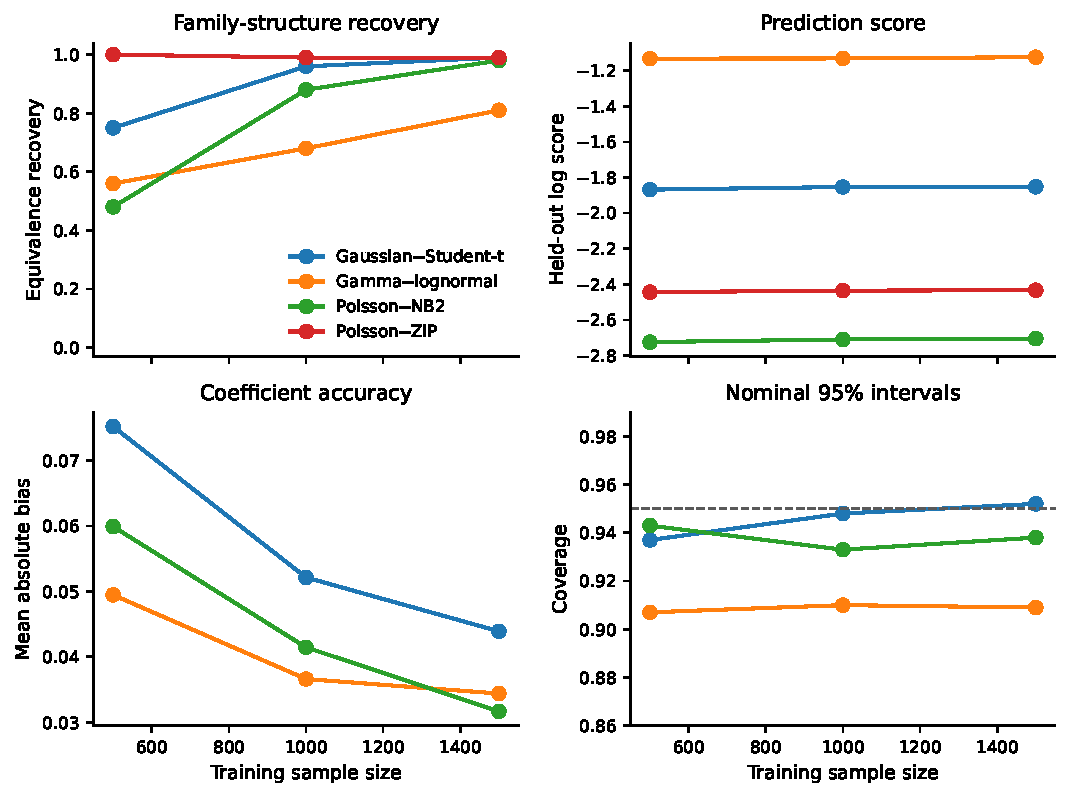
\includegraphics[width=\textwidth]{figures/simulation_sample_size.pdf}
\caption{Scenario A and C sample-size behavior.  The upper panels show
equivalence-class family recovery and held-out log score for the
BIC-selected model; the lower panels show analytical-Louis mean absolute bias
and nominal 95\% Wald coverage.  Scenario A did not save root mean squared
error by sample size, so the prediction panel reports the saved held-out log
score.}
\label{fig:simulation_sample_size}
\end{figure}

\subsubsection{Family-tuple recovery and predictive leaderboards}

Table~\ref{tab:model_selection} summarizes structural recovery.  Strict
recovery of Gaussian--Student-$t$ increases from 0.75 to 0.99, while recovery of
the more overlapping Gamma--lognormal pair increases from 0.56 to 0.81.  The
Poisson--ZIP tuple is recovered in 99--100\% of replications.  For
Poisson--NB2, strict recovery is zero because the selected representation is
typically NB2--NB2 with one dispersion near the Poisson boundary; recovery of
the corresponding equivalence class increases from 0.48 to 0.98.

\begin{table}[t]
\centering
\caption{Scenario A: family-tuple recovery and top-ten inclusion rates.  The
equivalence rate accounts for the boundary representations described in the
text.  Prediction ranks use held-out average log likelihood.}
\label{tab:model_selection}
\small
\begin{tabular}{llrrrr}
\toprule
Generating tuple & \(n\) & Strict & Equivalent & BIC top 10 & Prediction top 10 \\
\midrule
Gaussian--Student-\(t\) & 500  & .75 & .75 & 1.00 & 1.00 \\
 & 1000 & .96 & .96 & 1.00 & .99 \\
 & 1500 & .99 & .99 & 1.00 & .98 \\
Gamma--lognormal & 500  & .56 & .56 & 1.00 & .98 \\
 & 1000 & .68 & .68 & .98 & .98 \\
 & 1500 & .81 & .81 & .95 & .95 \\
Poisson--NB2 & 500  & .00 & .48 & 1.00 & 1.00 \\
 & 1000 & .00 & .88 & 1.00 & 1.00 \\
 & 1500 & .00 & .98 & 1.00 & 1.00 \\
Poisson--ZIP & 500  & 1.00 & 1.00 & 1.00 & 1.00 \\
 & 1000 & .99 & .99 & 1.00 & 1.00 \\
 & 1500 & .99 & .99 & 1.00 & 1.00 \\
\bottomrule
\end{tabular}
\end{table}

The BIC winner is also the held-out likelihood winner in only 18--72\% of
replications, depending on the design and sample size.  This disagreement is
expected: BIC targets a parsimonious generative representation, whereas
held-out likelihood can favor a nearby, more flexible candidate.  The
leaderboard result is more informative than exact agreement: the true or
equivalent tuple appears among the ten best models under both criteria with
probability at least 0.95 in all reported settings.

\subsubsection{Component-specific variable selection}

Table~\ref{tab:variable_selection} reports Scenario B.  The unpenalized model
retains virtually every inactive coefficient.  Lasso sharply reduces false
selection while retaining most signals: its true-positive rate ranges from
0.717 to 1.000 and its false-positive rate from 0.152 to 0.297.  Elastic net is
less sparse and retains slightly more signal in the Gamma--lognormal and
Poisson--ZIP designs.  The Gamma--lognormal example exposes the main trade-off:
lasso gives the cleanest support but loses held-out likelihood relative to the
dense fit.  Penalization should therefore be viewed as structural
regularization, not as a guarantee of improved point prediction.

\begin{table}[t]
\centering
\caption{Scenario B: variable-selection performance at \(n=1000\).  TPR,
FPR, and FDR are true-positive, false-positive, and false-discovery rates,
respectively.
Selected is the mean total model size across two components.}
\label{tab:variable_selection}
\small
\begin{tabular}{llrrrrr}
\toprule
Generating tuple & Penalty & TPR & FPR & FDR & Selected & Test log score \\
\midrule
Gaussian--Student-\(t\) & None & 1.000 & .998 & .750 & 39.95 & -1.919 \\
 & Lasso & 1.000 & .222 & .388 & 16.66 & -1.915 \\
 & Elastic net & 1.000 & .524 & .602 & 25.72 & -1.917 \\
Gamma--lognormal & None & 1.000 & .995 & .749 & 39.84 & -1.152 \\
 & Lasso & .717 & .152 & .289 & 11.74 & -1.170 \\
 & Elastic net & .766 & .276 & .494 & 15.93 & -1.165 \\
Poisson--ZIP & None & 1.000 & .997 & .749 & 39.92 & -2.477 \\
 & Lasso & .975 & .297 & .452 & 18.67 & -2.473 \\
 & Elastic net & .985 & .383 & .520 & 21.33 & -2.473 \\
\bottomrule
\end{tabular}
\end{table}

\begin{figure}[t]
\centering
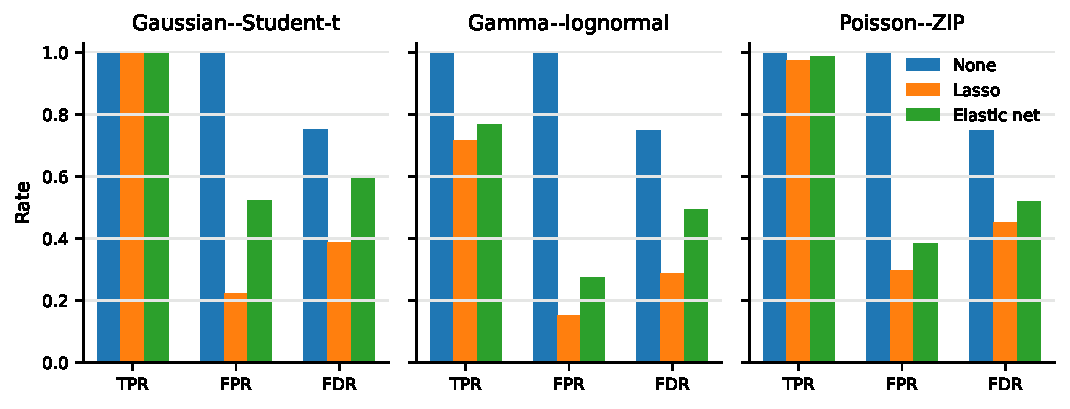
\includegraphics[width=\textwidth]{figures/variable_selection.pdf}
\caption{Scenario B component-specific variable selection.  The unpenalized
fit retains nearly all inactive coefficients, whereas lasso and elastic net
substantially reduce false-positive and false-discovery rates while preserving
most active coefficients.}
\label{fig:variable_selection}
\end{figure}

\subsubsection{Analytical Louis inference}

Analytical Louis and numerical-Hessian summaries agree to the displayed
precision in every Scenario C configuration, and both calculations succeed in
all replications.  Table~\ref{tab:louis_coverage} reports the analytical
results.  Coverage approaches 0.95 in the Gaussian--Student-$t$ design and
stays between 0.933 and 0.943 for Poisson--ZIP.  Gamma--lognormal has persistent
coverage near 0.91 despite agreement between the two information calculations.
We interpret this as finite-sample undercoverage caused by overlapping
positive-support components, rather than a derivative error.  Bias, standard
errors, and interval length decrease with sample size.

\begin{table}[t]
\centering
\caption{Scenario C: analytical Louis inference across regression
coefficients.  SE denotes standard error, and intervals are nominal 95\% Wald
intervals.}
\label{tab:louis_coverage}
\small
\begin{tabular}{lrrrrr}
\toprule
Generating tuple & \(n\) & Mean absolute bias & Mean SE & Coverage & CI length \\
\midrule
Gaussian--Student-\(t\) & 500  & .075 & .093 & .937 & .363 \\
 & 1000 & .052 & .065 & .948 & .254 \\
 & 1500 & .044 & .054 & .952 & .213 \\
Gamma--lognormal & 500  & .049 & .043 & .907 & .168 \\
 & 1000 & .037 & .030 & .910 & .119 \\
 & 1500 & .034 & .025 & .909 & .097 \\
Poisson--ZIP & 500  & .060 & .071 & .943 & .280 \\
 & 1000 & .041 & .049 & .933 & .192 \\
 & 1500 & .032 & .039 & .938 & .151 \\
\bottomrule
\end{tabular}
\end{table}

\subsection{Applications}
\label{sec:applications}

The two applications are reported using the same empirical template.  For each
dataset we summarize the model-search leaderboard, held-out log score,
root mean squared error (RMSE), mean absolute error (MAE), fitted mixture
weights, and component-specific active sets.  The RAND analysis additionally
includes a participant bootstrap because it is the stronger independent count
example and has a final fixed family pair validated across splits.

\begin{figure}[t]
\centering
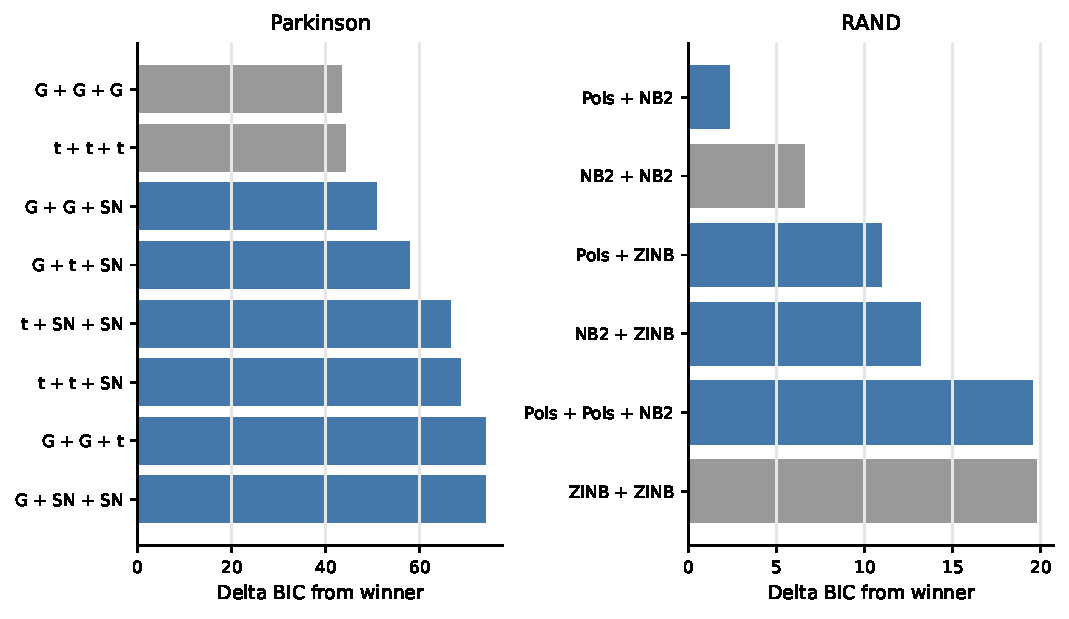
\includegraphics[width=\textwidth]{figures/application_leaderboards.pdf}
\caption{Application leaderboards by BIC.  Bars show the BIC difference from
the best converged model in each application; blue bars are non-identical
family tuples and gray bars are identical-family tuples.  BIC denotes the
Bayesian information criterion.}
\label{fig:application_leaderboards}
\end{figure}

\begin{figure}[t]
\centering
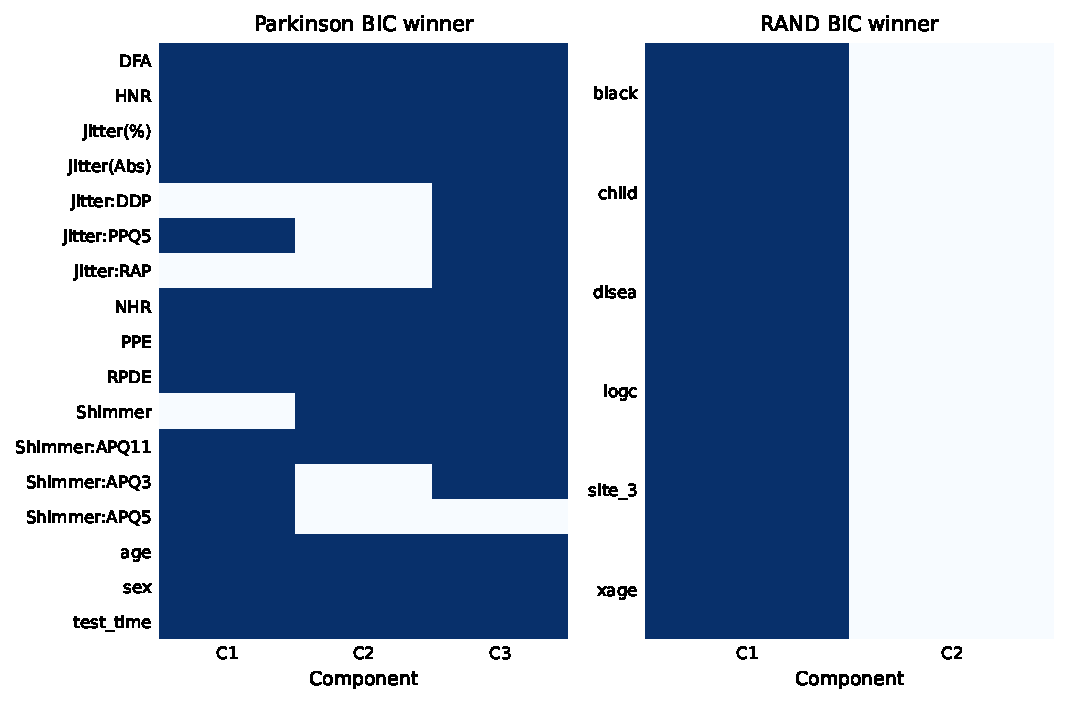
\includegraphics[width=\textwidth]{figures/application_supports.pdf}
\caption{Component-specific active supports for the BIC-selected application
models.  Dark cells indicate selected covariates.  The RAND support is
intercept-only in the NB2 component, while the Parkinson fit has partially
shared and partially component-specific voice-measure supports.}
\label{fig:application_supports}
\end{figure}

\subsubsection{Parkinson's telemonitoring}

The Parkinson's telemonitoring data contain 5,875 home voice recordings from
42 participants with early-stage Parkinson's disease
\citep{uci2009parkinsons,tsanas2010parkinsons}.  The response is the logarithm
of total Unified Parkinson's Disease Rating Scale (UPDRS).  Candidate predictors
include age, sex, time since recruitment, and 16 jitter, shimmer, noise, and
nonlinear voice measures.  We searched Gaussian, Student-$t$, and skew-normal
families with one to three components and a nine-value penalty grid.  A random
subset of 2,000 recordings was used for fitting and 1,000 for evaluation.
Consequently, the reported prediction scores assess new recordings from the
observed cohort rather than generalization to unseen participants.

Among 319 converged candidate fits, BIC selected a three-component
Student-$t$--skew-normal--skew-normal model with weights
\((0.475,0.229,0.296)\).  Its BIC was 1452.2, an improvement of 416.4 over
the best one-component model and 43.4 over the best converged identical-family
mixture.  The selected components retained 14, 12, and 16 predictors.  Eleven
predictors were common to all components, while six entered only a subset.
The differences involved jitter and shimmer summaries in particular: the third
component retained RAP, PPQ5, and DDP jitter measures, whereas the second
component omitted them and retained a smaller voice-feature set.

\begin{table}[t]
\centering
\caption{Parkinson's analysis: representative converged models.  SN denotes
skew normal.  Log score, RMSE, and MAE are evaluated on 1,000 held-out
recordings.}
\label{tab:parkinsons}
\small
\resizebox{\textwidth}{!}{%
\begin{tabular}{llrrrrrrr}
\toprule
Role & Family tuple & \(K\) & \(\lambda\) & BIC & Log score & RMSE/MAE & Weights & Active counts \\
\midrule
BIC winner & Student-\(t\)+SN+SN & 3 & 20 & 1452.2 & -297.3 & .392/.305 & .475/.229/.296 & 14/12/16 \\
Best identical BIC & Gaussian+Gaussian+Gaussian & 3 & 20 & 1495.6 & -287.3 & .385/.300 & .442/.079/.479 & 13/13/14 \\
Best one component & Student-\(t\) & 1 & 20 & 1868.6 & -441.3 & .384/.296 & 1.000 & 16 \\
Best log score & Gaussian+Gaussian+SN & 3 & 20 & 1503.0 & -286.8 & .385/.300 & .079/.440/.481 & 13/13/14 \\
Best RMSE & Gaussian+Student-\(t\) & 2 & 5 & 1818.3 & -402.1 & .382/.296 & .667/.333 & 17/18 \\
\bottomrule
\end{tabular}}
\end{table}

The BIC and held-out likelihood leaders are both non-identical, although they
select different tuples.  Mean prediction tells a weaker story: the best RMSE
improves only marginally on simpler models.  The application therefore supports
distributional heterogeneity and component-specific support more clearly than
it supports a large gain in conditional-mean prediction.

\subsubsection{RAND health-utilization counts}

The RAND Health Insurance Experiment data contain medical utilization,
insurance, demographic, and health-status variables
\citep{deb2002health,cameron2005microeconometrics}.  To avoid repeated-record
dependence, we retained the earliest record for each of 5,912 participants and
modeled the number of non-physician visits.  The search included Poisson, NB2,
ZIP, and ZINB families; one to three components; ten penalty values; and two
initialization schemes.  Fifty predictors were screened within each training
sample.  We performed three independent 80/20 participant splits and then an
exhaustive fit to all participants.

The Poisson--NB2 tuple was the BIC winner in every split
(Table~\ref{tab:rand_splits}).  Its average BIC advantage was 429.0 over the
best one-component model and 9.77 over the best identical-family mixture.
Weights were stable at approximately 0.83 and 0.17.  Held-out log likelihood
improved substantially over the one-component model but was essentially tied
with NB2--NB2.  RMSE and MAE did not improve, underscoring that the gain concerns
the predictive distribution rather than its mean.

\begin{table}[t]
\centering
\caption{RAND split validation for the BIC-selected Poisson--NB2 mixture.
Log score is held-out average log likelihood per participant.  The BIC
improvement columns are positive when Poisson--NB2 improves on the indicated
comparator.}
\label{tab:rand_splits}
\small
\resizebox{\textwidth}{!}{%
\begin{tabular}{rrrrrrrrr}
\toprule
Split & \(\lambda\) & BIC & vs. one component & vs. identical &
Log score & RMSE/MAE & Weights & Active counts \\
\midrule
1 & 50  & 6434.9 & 396.6 & 14.5 & -.642 & 3.006/.844 & .831/.169 & 12/0 \\
2 & 100 & 6472.1 & 483.1 & 11.3 & -.628 & 2.842/.867 & .831/.169 & 4/0 \\
3 & 100 & 6353.0 & 407.0 & 3.5  & -.683 & 1.926/.808 & .836/.164 & 5/0 \\
\bottomrule
\end{tabular}}
\end{table}

In the full-data search, Poisson--NB2 again ranked first (BIC 7950.6), followed
by Poisson--ZINB (7954.4) and NB2--NB2 (7955.2).  The best one-component model
had BIC 8504.9.  In the NB2--NB2 comparator, the first estimated dispersion was
\(\exp(-8.52)\), effectively the Poisson boundary.  Thus the selected tuple
is best interpreted as a parsimonious Poisson-like majority component plus a
strongly overdispersed NB2 minority, not as proof that the broader NB2 family
cannot represent both groups.

The full-data penalized fit selected age, child status, disease burden, Black
race, log coinsurance, and the site-3 indicator in the Poisson component; the
NB2 component was intercept-only.  An unpenalized refit conditional on that
support gave weights \((0.841,0.159)\) and NB2 dispersion 10.36.  The reduced
analytical Louis information had dimension and rank 10, minimum eigenvalue
1.28, and condition number 1439.  Conditional Louis intervals excluded zero
for all six coefficients, but those intervals do not account for the selected
support.

We therefore used 500 participant bootstrap samples as the primary uncertainty
analysis.  Each sample repeated predictor screening, penalty tuning, support
selection, and the constrained post-lasso refit while holding the independently
validated family tuple fixed.  All 500 runs completed.  The minority weight had
a percentile interval of \((0.132,0.191)\), and NB2 dispersion had interval
\((4.33,12.16)\).  Table~\ref{tab:rand_bootstrap} shows that age and site 3
were the most stable covariates.  Intervals include zero when the resampled
selection pipeline omits a variable; log coinsurance also showed sign
instability.

\begin{table}[t]
\centering
\caption{RAND selection-aware bootstrap for coefficients in the Poisson
component.  Bootstrap SE denotes bootstrap standard error.  Intervals are
percentile intervals from the complete resampled selection-and-refit pipeline.}
\label{tab:rand_bootstrap}
\small
\begin{tabular}{lrrrr}
\toprule
Covariate & Selection frequency & Estimate & Bootstrap SE & 95\% interval \\
\midrule
Age & 1.000 & .221 & .079 & (.094, .400) \\
Site 3 & .988 & .210 & .058 & (.003, .247) \\
Log coinsurance & .886 & -.319 & .148 & (-.369, .147) \\
Disease burden & .868 & .127 & .045 & (.000, .152) \\
Child & .796 & -.191 & .173 & (-.288, .000) \\
Black & .682 & -.136 & .084 & (-.254, .000) \\
\bottomrule
\end{tabular}
\end{table}

Support selection was less stable than family selection.  The bootstrap chose
\(\lambda=50\) in 67.4\% of samples and \(\lambda=100\) in 19.6\%, and
the median active-set sizes were 16 and 2 rather than the full-data 6 and 0.
Accordingly, the six-variable support is a parsimonious full-data
representation, not a uniquely determined scientific model.

\section{Discussion and conclusions}
\label{sec:discussion}

Allowing response families to vary across latent regression components
addresses a simple but consequential limitation of conventional mixture GLMs.
In both simulations and applications, non-identical tuples distinguish
heterogeneity in regression effects from heterogeneity in dispersion, skewness,
tail weight, and zero inflation.  The framework remains modular: component
families contribute their own likelihood, link, nuisance update, and derivative
block, while EM responsibilities and Louis' missing-information correction are
shared.

The numerical results support three conclusions.  First, family-tuple recovery
improves with sample size, but exact labels are not always the right target when
families meet at a boundary.  Second, componentwise penalization can greatly
reduce false selection, although sparse support and optimal prediction need not
coincide.  Third, analytical Louis information reproduces numerical-Hessian
inference while avoiding a fragile high-dimensional differentiation step.  The
RAND analysis combines these points: a Poisson-like majority and an
overdispersed minority are reproducible across splits, whereas individual
covariates have varying selection stability.

Several limitations define useful directions for further work.  The regular
theory conditions on a fixed, identifiable family tuple with interior
parameters and nonsingular information.  It does not justify ordinary Wald
inference after selecting the number of components, family tuple, or active
set.  Singular criteria, selective inference, and family-selection bootstrap
procedures are important extensions \citep{drton2017sbic,leeb2005selection}.
The RAND bootstrap repeats variable selection but conditions on the family pair;
its intervals should be read accordingly.

The empirical analyses use a common penalty parameter across components.
Because effective component sample sizes can differ, a common absolute penalty
may shrink a small component more strongly.  Component-specific or
effective-sample-size-adjusted tuning is a natural extension.  The
intercept-only NB2 support in the full RAND fit is therefore not evidence that
all measured covariates are irrelevant in that component; the bootstrap
selection frequencies convey the appropriate uncertainty.

The Parkinson application contains repeated recordings.  Its recording-level
split measures interpolation to additional recordings from the observed
participant cohort and should not be interpreted as new-participant validation.
Grouped likelihoods, participant-level cross-validation, random effects, and
cluster bootstrap inference would extend the model to longitudinal data.
Finally, exhaustive family search is combinatorial and EM remains sensitive to
local modes.  Better warm starts, branch-and-bound search, parallel screening,
and covariate-dependent mixing weights in the spirit of mixture-of-experts
models are promising computational developments.

Within these boundaries, component-specific response families offer a useful
middle ground between a rigid homogeneous-family mixture and a fully
nonparametric conditional density model.  They preserve interpretable
component regressions, permit sparse component-specific scientific summaries,
and support likelihood-based uncertainty calculations when the fitted model is
regular.  The central practical recommendation is equally important: report
family selection, prediction, support stability, and fixed-model uncertainty as
distinct objects rather than expecting one ranking or standard error to answer
all four questions.

\section*{Data and code availability}

The Python implementation, simulation scripts, data-preparation scripts, job
specifications, and processed result tables used in this paper are included in
the accompanying reproducibility archive and the project repository at
\url{https://github.com/samyajoypal/mixglm}.  The file
\texttt{REPRODUCIBILITY.md} lists the source files and saved artifacts needed
to rebuild the tables and figures.  The two applications use publicly
available RAND Health Insurance Experiment and UCI Parkinson's telemonitoring
data.

\clearpage
\appendix

\section{Analytical Louis Blocks and Weighted M-Step Equations}
\label{app:louis_mstep}

This appendix records the analytical ingredients used by the observed
information and by the componentwise maximization step.  The main text gives
the finite-mixture Louis identity and the chain rule that maps a
family-specific derivative block into regression coordinates.  We now list the
family blocks in the \((\mu,\gamma)\) coordinates used by the optimizer, and
then state the weighted M-step equations solved inside the generalized
expectation-maximization algorithm.

\subsection{Notation for family-specific Louis blocks}

For one observation from one component, write
\[
    \ell=\log f(y;\mu,\gamma),\qquad
    a_\mu=\frac{\partial \ell}{\partial\mu},\qquad
    b_{\mu\mu}=\frac{\partial^2\ell}{\partial\mu^2},
\]
\[
    a_\gamma=\frac{\partial\ell}{\partial\gamma},\qquad
    B_{\gamma\gamma}=
    \frac{\partial^2\ell}{\partial\gamma\,\partial\gamma^\top},
    \qquad
    b_{\mu\gamma}=
    \frac{\partial^2\ell}{\partial\mu\,\partial\gamma}.
\]
Cross-derivatives not displayed are zero.  Positive nuisance parameters are
differentiated after log transformation, and probabilities constrained to
\((0,1)\) are differentiated after the logit transformation.  The functions
\(\psi\) and \(\psi_1\) denote the digamma and trigamma functions.

\paragraph{Gaussian.}
For \(N(\mu,\sigma^2)\), let \(v=\sigma^2=\exp(s)\) and \(r=y-\mu\).  Then
\[
    a_\mu=r/v,\qquad b_{\mu\mu}=-1/v,
\]
\[
    a_s=-1/2+r^2/(2v),\qquad
    B_{ss}=-r^2/(2v),\qquad
    b_{\mu s}=-r/v.
\]

\paragraph{Student-\(t\).}
Let \(\sigma=\exp(a)\), \(\nu=2+\exp(b)\), \(w=\exp(b)\),
\(r=y-\mu\), \(D=\nu\sigma^2+r^2\), \(u=r^2/\sigma^2\), and
\(q=1+u/\nu\).  Then
\[
    a_\mu=\frac{(\nu+1)r}{D},\qquad
    b_{\mu\mu}=\frac{(\nu+1)(r^2-\nu\sigma^2)}{D^2},
\]
\[
    a_a=-1+\frac{(\nu+1)r^2}{D},\qquad
    B_{aa}=-\frac{2(\nu+1)r^2\nu\sigma^2}{D^2},\qquad
    b_{\mu a}=-\frac{2(\nu+1)r\nu\sigma^2}{D^2}.
\]
With
\[
    L_\nu=
    \frac12\psi\!\left(\frac{\nu+1}{2}\right)
    -\frac12\psi\!\left(\frac{\nu}{2}\right)
    -\frac{1}{2\nu}
    -\frac12\log q
    +\frac{(\nu+1)u}{2\nu(\nu+u)}
\]
and
\[
    L_{\nu\nu}=
    \frac14\psi_1\!\left(\frac{\nu+1}{2}\right)
    -\frac14\psi_1\!\left(\frac{\nu}{2}\right)
    +\frac{1}{2\nu^2}
    +\frac{u}{2\nu(\nu+u)}
    +\frac{\frac12u\nu(\nu+u)-\frac12u(\nu+1)(2\nu+u)}
           {\{\nu(\nu+u)\}^2},
\]
the transformed degree-of-freedom derivatives are
\[
    a_b=wL_\nu,\qquad B_{bb}=wL_\nu+w^2L_{\nu\nu},
\]
\[
    b_{\mu b}=\frac{w\,r(r^2-\sigma^2)}{D^2},\qquad
    B_{ab}=\frac{w\,r^2(r^2-\sigma^2)}{D^2}.
\]

\paragraph{Poisson.}
For \(Y\sim\operatorname{Poisson}(\mu)\),
\[
    a_\mu=y/\mu-1,\qquad b_{\mu\mu}=-y/\mu^2.
\]

\paragraph{Negative binomial with quadratic variance.}
For the NB2 parameterization \(\operatorname{Var}(Y)=\mu+\alpha\mu^2\), let
\(\rho=\log\alpha\), \(r=\alpha^{-1}=\exp(-\rho)\), and \(A=r+\mu\).  Then
\[
    a_\mu=\frac{y}{\mu}-\frac{r+y}{A},\qquad
    b_{\mu\mu}=-\frac{y}{\mu^2}+\frac{r+y}{A^2}.
\]
Define
\[
    L_r=\psi(y+r)-\psi(r)+\log r+1-\log A-\frac{r+y}{A},
\]
\[
    L_{rr}=
    \psi_1(y+r)-\psi_1(r)+1/r-1/A-(\mu-y)/A^2.
\]
Then
\[
    a_\rho=-rL_r,\qquad
    B_{\rho\rho}=rL_r+r^2L_{rr},\qquad
    b_{\mu\rho}=r(\mu-y)/A^2.
\]

\paragraph{Gamma.}
For the mean-shape Gamma model with shape \(\kappa=\exp(a)\),
\[
    \ell=(\kappa-1)\log y-\kappa y/\mu-\log\Gamma(\kappa)
    -\kappa\log\mu+\kappa\log\kappa .
\]
Let
\[
    L_\kappa=\log y-y/\mu-\psi(\kappa)-\log\mu+\log\kappa+1,
    \qquad
    L_{\kappa\kappa}=-\psi_1(\kappa)+1/\kappa .
\]
Then
\[
    a_\mu=\kappa(y-\mu)/\mu^2,\qquad
    b_{\mu\mu}=\kappa(\mu-2y)/\mu^3,
\]
\[
    a_a=\kappa L_\kappa,\qquad
    B_{aa}=\kappa L_\kappa+\kappa^2L_{\kappa\kappa},\qquad
    b_{\mu a}=a_\mu.
\]

\paragraph{Exponential.}
For the exponential distribution parameterized by its mean,
\[
    a_\mu=(y-\mu)/\mu^2,\qquad b_{\mu\mu}=(\mu-2y)/\mu^3.
\]

\paragraph{Lognormal.}
For the lognormal component, \(\mu\) denotes log-location.  Let
\(\sigma=\exp(a)\) and \(r=\log y-\mu\).  Then
\[
    a_\mu=r/\sigma^2,\qquad b_{\mu\mu}=-1/\sigma^2,
\]
\[
    a_a=-1+r^2/\sigma^2,\qquad
    B_{aa}=-2r^2/\sigma^2,\qquad
    b_{\mu a}=-2r/\sigma^2.
\]

\paragraph{Inverse Gaussian.}
For mean \(\mu\) and \(\lambda=\exp(a)\), let
\[
    A=(y-\mu)^2/(2\mu^2y).
\]
Then
\[
    a_\mu=\lambda(y-\mu)/\mu^3,\qquad
    b_{\mu\mu}=\lambda(2\mu-3y)/\mu^4,
\]
\[
    a_a=1/2-\lambda A,\qquad
    B_{aa}=-\lambda A,\qquad
    b_{\mu a}=a_\mu.
\]

\paragraph{Bernoulli and geometric.}
For Bernoulli success probability \(\mu\),
\[
    a_\mu=\frac{y}{\mu}-\frac{1-y}{1-\mu},\qquad
    b_{\mu\mu}=-\frac{y}{\mu^2}-\frac{1-y}{(1-\mu)^2}.
\]
For the geometric law on \(\{0,1,\ldots\}\) parameterized by mean \(\mu\),
\[
    a_\mu=y/\mu-(y+1)/(1+\mu),\qquad
    b_{\mu\mu}=-y/\mu^2+(y+1)/(1+\mu)^2.
\]

\paragraph{Beta.}
For the beta mean-precision parameterization, let
\(\phi=\exp(a)\), \(A=\mu\phi\), and \(B=(1-\mu)\phi\).  Define
\[
    G=-\psi(A)+\psi(B)+\log y-\log(1-y),
\]
\[
    L_\phi=
    \psi(\phi)-\mu\psi(A)-(1-\mu)\psi(B)
    +\mu\log y+(1-\mu)\log(1-y),
\]
\[
    L_{\phi\phi}=
    \psi_1(\phi)-\mu^2\psi_1(A)-(1-\mu)^2\psi_1(B).
\]
Then
\[
    a_\mu=\phi G,\qquad
    b_{\mu\mu}=-\phi^2\{\psi_1(A)+\psi_1(B)\},
\]
\[
    a_a=\phi L_\phi,\qquad
    B_{aa}=\phi L_\phi+\phi^2L_{\phi\phi},
\]
\[
    b_{\mu a}=
    \phi G+\phi^2\{-\mu\psi_1(A)+(1-\mu)\psi_1(B)\}.
\]

\paragraph{Zero-inflated Poisson.}
Let \(\zeta=\operatorname{logit}(\theta)\),
\(\dot\theta=\theta(1-\theta)\).  For \(y>0\),
\[
    a_\mu=y/\mu-1,\qquad b_{\mu\mu}=-y/\mu^2,\qquad
    a_\zeta=-\theta,\qquad B_{\zeta\zeta}=-\dot\theta.
\]
For \(y=0\), let \(e=\exp(-\mu)\),
\[
    A=\theta+(1-\theta)e,\quad B=(1-\theta)e,\quad
    C=\dot\theta(1-e),\quad
    C_\zeta=\dot\theta(1-2\theta)(1-e).
\]
Then
\[
    a_\mu=-B/A,\qquad b_{\mu\mu}=B\theta/A^2,
\]
\[
    a_\zeta=C/A,\qquad
    B_{\zeta\zeta}=(C_\zeta A-C^2)/A^2,\qquad
    b_{\mu\zeta}=(\dot\theta eA+CB)/A^2.
\]

\paragraph{Zero-inflated negative binomial.}
For positive counts, use the NB2 block and add
\[
    a_\zeta=-\theta,\qquad B_{\zeta\zeta}=-\theta(1-\theta).
\]
For \(y=0\), let \(p_0=\{r/(r+\mu)\}^r\),
\[
    A=\theta+(1-\theta)p_0,\quad
    C=\dot\theta(1-p_0),\quad
    C_\zeta=\dot\theta(1-2\theta)(1-p_0).
\]
Let \(g_j\) and \(H_{j\ell}\) be the NB2 score and Hessian entries for
\(\log p_0\) in \(j,\ell\in\{\mu,\rho\}\).  Define
\[
    A_j=(1-\theta)p_0g_j,\qquad
    A_{j\ell}=(1-\theta)p_0(H_{j\ell}+g_jg_\ell),\qquad
    A_{j\zeta}=-\dot\theta p_0g_j .
\]
Then
\[
    a_j=A_j/A,\qquad
    B_{j\ell}=(A_{j\ell}A-A_jA_\ell)/A^2,
\]
\[
    a_\zeta=C/A,\qquad
    B_{\zeta\zeta}=(C_\zeta A-C^2)/A^2,\qquad
    B_{j\zeta}=(A_{j\zeta}A-A_jC)/A^2.
\]

\paragraph{Skew normal.}
For the Azzalini skew-normal component, let \(\omega=\exp(a)\),
\(\alpha\) be the shape, \(z=(y-\mu)/\omega\), and \(t=\alpha z\).
With \(M(t)=\varphi(t)/\Phi(t)\) and
\(M'(t)=-M(t)\{t+M(t)\}\), set
\[
    \ell_z=-z+\alpha M(t),\quad
    \ell_{zz}=-1+\alpha^2M'(t),\quad
    \ell_{z\alpha}=M(t)+\alpha zM'(t).
\]
Then
\[
    a_\mu=-\ell_z/\omega,\qquad
    b_{\mu\mu}=\ell_{zz}/\omega^2,
\]
\[
    a_a=-1-z\ell_z,\qquad
    a_\alpha=zM(t),
\]
\[
    B_{aa}=z\ell_z+z^2\ell_{zz},\qquad
    B_{\alpha\alpha}=z^2M'(t),\qquad
    B_{a\alpha}=-z\ell_{z\alpha},
\]
\[
    b_{\mu a}=(\ell_z+z\ell_{zz})/\omega,\qquad
    b_{\mu\alpha}=-\ell_{z\alpha}/\omega.
\]

\subsection{Weighted M-step equations}
\label{app:mstep}

At an expectation-maximization iteration, component \(k\) receives weights
\(w_i=\tau_{ik}\).  Its regression and nuisance update solves
\[
    (\beta_k^{+},\gamma_k^{+})
    \in
    \argmax_{\beta,\gamma}
    \left\{
    \sum_{i=1}^n w_i
    \ell_{d_k}\{y_i;h_{d_k}(x_i^\top\beta),\gamma\}
    -
    \lambda_k\rho_k(\beta_{-0})
    \right\}.
\]
The intercept is not penalized.  With
\[
    U_{\eta i}=a_{\mu i}\dot h_i,\qquad
    J_{\eta i}=-
    \{b_{\mu\mu,i}\dot h_i^2+a_{\mu i}\ddot h_i\},
\]
the unpenalized score and negative Hessian for the regression coordinates are
\[
    U_\beta(\beta,\gamma)=\sum_{i=1}^n w_i x_i U_{\eta i},
    \qquad
    J_{\beta\beta}(\beta,\gamma)=
    \sum_{i=1}^n w_i x_ix_i^\top J_{\eta i}.
\]
Thus a Newton or iteratively reweighted least-squares step has working
response
\[
    z_i=x_i^\top\beta+U_{\eta i}/J_{\eta i}
\]
and working weight \(w_iJ_{\eta i}\), whenever \(J_{\eta i}>0\).  The
unpenalized active-coordinate update is
\[
    \beta_{\mathcal A}^{+}
    =
    \argmin_b
    \frac12
    \sum_{i=1}^n w_iJ_{\eta i}
    (z_i-x_{i,\mathcal A}^\top b)^2.
\]
For a ridge penalty this becomes the usual penalized normal equation, with no
ridge term on the intercept.  For a lasso penalty, the coordinatewise quadratic
approximation gives the soft-thresholding update
\[
    \beta_j^{+}
    =
    \frac{
    S\left\{
    \sum_i w_iJ_{\eta i}x_{ij}
    \left(z_i-\sum_{\ell\neq j}x_{i\ell}\beta_\ell\right),
    \lambda_k
    \right\}}
    {\sum_i w_iJ_{\eta i}x_{ij}^2},
    \qquad j>0,
\]
where \(S(u,\lambda)=\operatorname{sign}(u)(|u|-\lambda)_+\).  Elastic-net
updates replace the denominator by
\(\sum_i w_iJ_{\eta i}x_{ij}^2+\lambda_k(1-\alpha)\) and use
\(\lambda_k\alpha\) in the threshold.

The nuisance update is low-dimensional and uses the same weighted likelihood.
For example, the Gaussian variance has the closed-form update
\[
    \hat\sigma_k^2
    =
    \frac{\sum_i w_i(y_i-x_i^\top\beta_k)^2}{\sum_i w_i}.
\]
For NB2 dispersion, Gamma shape, Student-\(t\) scale and degrees of freedom,
zero-inflation probabilities, beta precision, and skew-normal shape and scale,
the update solves
\[
    U_\gamma(\beta,\gamma)=
    \sum_{i=1}^n w_i a_{\gamma i}=0
\]
by a scalar or low-dimensional Newton/L-BFGS step using the analytical
\(B_{\gamma\gamma}\) and \(b_{\mu\gamma}\) blocks above.  If the block update
increases the weighted penalized objective but is not globally maximized, the
outer algorithm is a generalized EM algorithm; the monotonicity theorem in the
main text applies under that explicit ascent condition.


\bibliographystyle{plainnat}
\bibliography{references}

\end{document}
